% !TEX root =../thesis-letomes.tex

\chapter{Results}
The main aim of the project was twofold: to examine whether or not ES was a reasonable method to apply in this problem space, and to create a mars mission simulator to compare it with the lunar case, under the expectation that the two problems would be more or less similar. We have accomplished both these things, certainly, even though they did not take the shape we were initially expecting. In this chapter we will examine the various threads of the project, to see where they ended up.

\section{Evolution Strategies' fitness for this problem space}
We implemented several versions of the fundamental ES concept, with different combinations of additions that have given good results in the literature. Certain additions had more impact than others, but no matter what variation we used, the results weren't exactly earth-shattering. The problem space has a fractured, fractal quality of very good solutions hiding among very bad ones. These solutions are not found in any particularly ingenious fashion by ES, nor by any gradient descent method, really. There are areas of good structure, where ES finds a local minimum just fine, but if the objective is simply to find a decent solution, then something naive like random guessing will also perform well, since the space is sufficiently dense with decent solutions. 

When we computed the problem space flattened to two dimensions by locking the burn-angle to 0, we gained valuable information and intuition about its shape. We are dealing with a heavily fractal space of ridges with a cross section of the approximate shape shown in figure \ref{fig:ridge_cross_section}

\begin{figure}[h]
    \centering
    \subfloat[The approximate cross-section of the ridges]{
        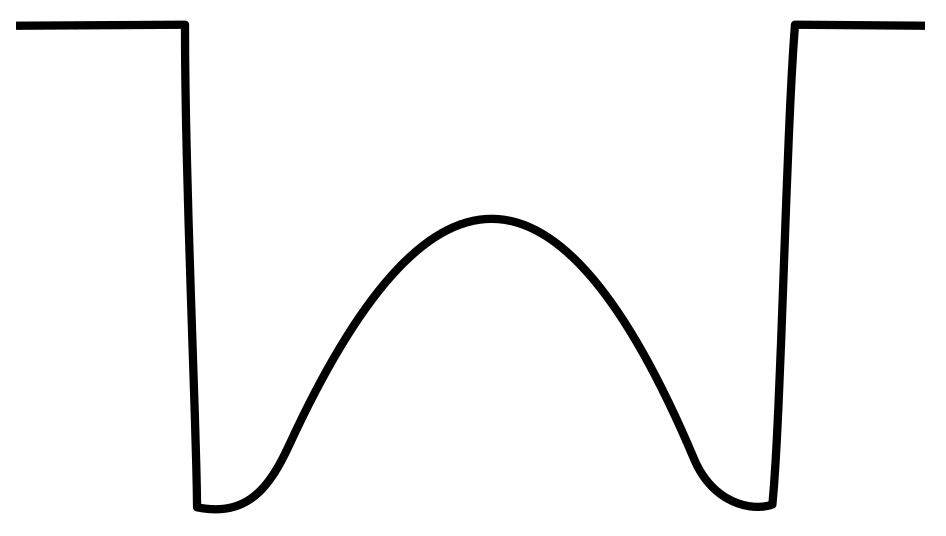
\includegraphics[width=0.46\linewidth]{fig/ridge_cross_section.png}
        \label{fig:ridge_cross_section}
    }
    \hfill
    \subfloat[a ridge in the problem space]{
        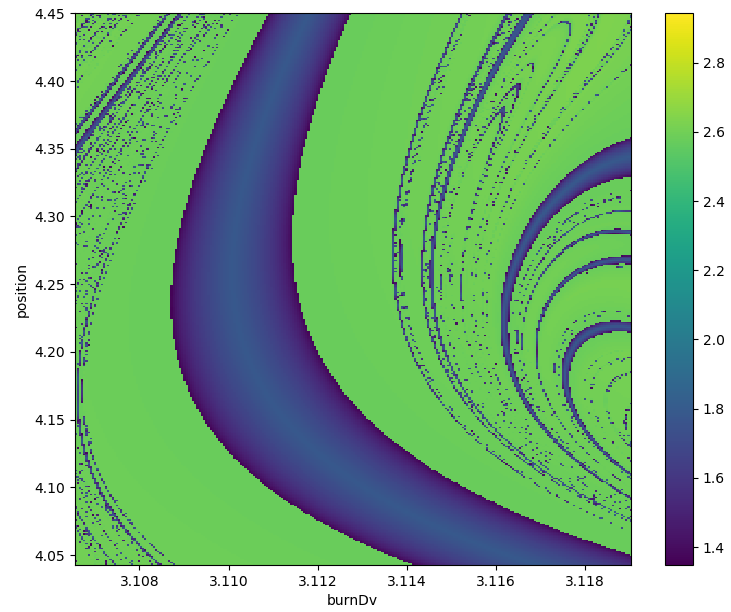
\includegraphics[width=0.46\linewidth]{fig/ridge.png}
        \label{fig:ridge}
    }
    \caption{The problem space is populated densely by ridges with the approximate cross-section seen in \ref{fig:ridge_cross_section}. There are infinitely many of these, if we extrapolate from what we have seen as we have zoomed in.}
\end{figure}

The fractal nature of the space heavily indicates that some variational optimization method would help. If we are to follow ridges of arbitrary width, we need to be able to scale our across-ridge variance down, so most of $\sigma\epsilon$ falls within the ridge we are following. See figure \ref{fig:confusioninfractalarea} and \ref{fig:esdivergingfromridge} for examples of the confusion that we see when we are looking at a fractal area. We did not extend the algorithm with proper variational training, but a 'fake' version of it, with a linearly declining $\sigma$ and a strategically chosen starting point gave us some promising signs. In figure \ref{fig:chilling_on_ridge}, this is implemented, and it lets us stay within the bounds of the ridge. We would need to implement this properly to make any conclusions. 

If a measure like this were added, we could use it as a meaningful stopping criterion as well. Once $\sigma$ is on the order of \num{1e-4} in the 'position' dimension for example, the required precision of the associated maneouvre is in the order of tenths of a second. This is not really a reasonable sensitivity for an actual Moon mission. Thus, when we take reality into account, we see that we can't really use solutions that are too granular. What we are looking for are patches of adjacent good solutions at a large enough scale that they allow \emph{some} flexibility in terms of when the maneouver is begun and how hard we burn.

\begin{figure}[h]
    \centering
    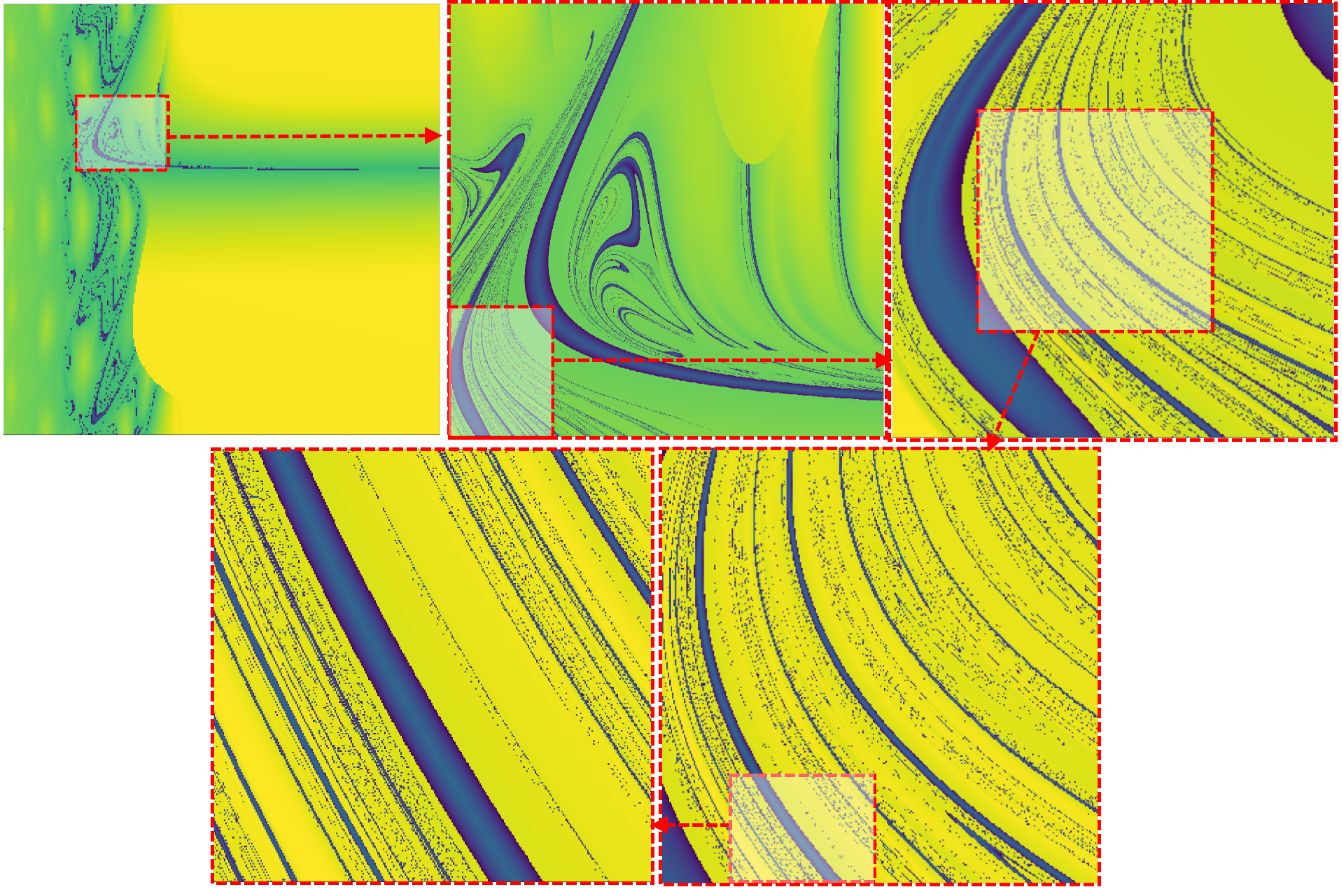
\includegraphics[width=\linewidth]{fig/consecutivezoom.png}
    \caption{Repeated zoom-ins on the problem space show regions of fractal ridges, all but necessitating some adaptive variance measure. }
    \label{fig:consecutivezoom}
\end{figure} 

\begin{figure}
    \centering
    \subfloat[The algorithm experiences confusion when it starts in a fractal area]{
        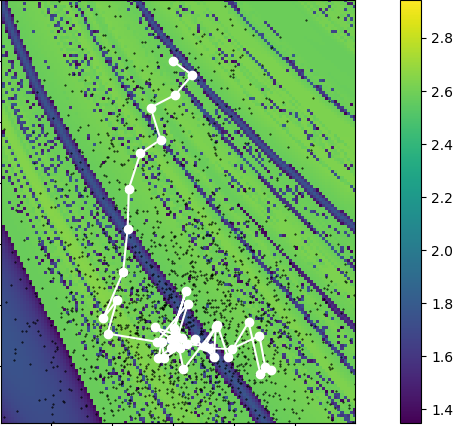
\includegraphics[width=0.46\linewidth]{fig/confusioninfractalarea}
        \label{fig:confusioninfractalarea}
    }
    \hfill
    \subfloat[Here we see the algorithm locating and settling in a ridge]{
        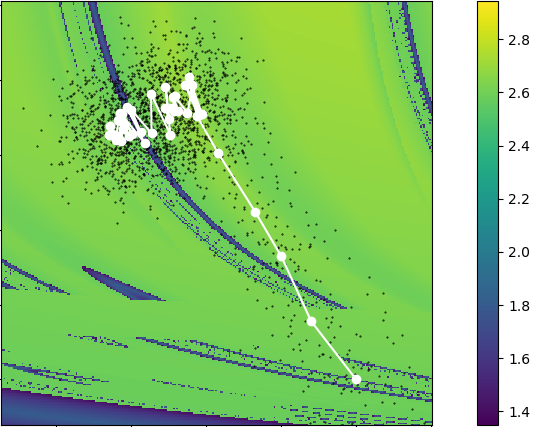
\includegraphics[width=0.46\linewidth]{fig/findingridge.PNG}
        \label{fig:findingridge}
    }
    \\
    \subfloat[We see that there is not much of a gradient along the ridges. This might indicate that a momentum-based strategy might be a valuabe addition, if we want to search the ridges properly. CMA-ES is also an interesting prospect, for the same reason.]{
        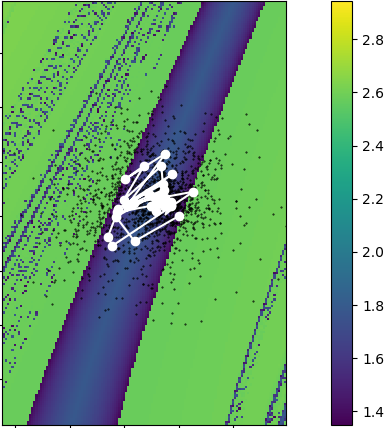
\includegraphics[width=0.46\linewidth]{fig/chilling_on_ridge.png}
        \label{fig:chilling_on_ridge}
    }
    \hfill
    \subfloat[The rate of separation of two infinitesimally perturbed versions of the long LETO]{
        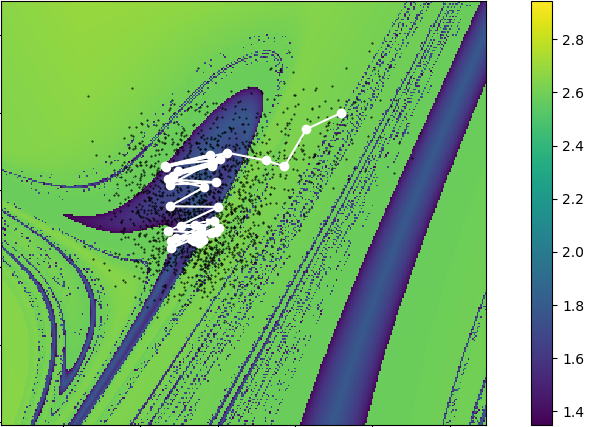
\includegraphics[width=0.46\linewidth]{fig/EScatchingridge.png}
        \label{fig:EScatchingridge}
    }
    \caption{Examples of some of the different types of transfers that are possible within the model. Each of these were taken as starting points, and simulated again with slightly perturbed starting conditions. The difference between these perturbations were then measured, and plotted in \textbf{b} and \textbf{d}, on a logarithmic scale. The slope of these plots is the lyapunov exponent. We can see that passing into a deep gravity well has a stabilizing effect on the chaos in the system.}
    \label{fig:lyapunov} 
\end{figure} 



\section{Finding LETOs to Mars}

\section{Stability of Trajectories: Lyapunov Exponent}
\subsection{Sensitivity analysis}

In our experiments, we found that our paths were diverging pretty heavily given relatively small changes to initial conditions. This was a concern in the original project as well, but was not fully explored then. It is important to quantify the chaotic nature of a system like this, since we are dealing with numerical simulation, which will always have some error associated with it. One takes steps to minimize such errors, often sacrificing computing performance to do so. However, if a system has an error of magnitude say \(\num{1e-8}\), and the system is so chaotic that errors of or \(\num{1e-9}\) at one point early in the trajectory effect meaningful changes further down the line, then the path is near invalid! Therefore, it is important to try to quantify the chaos of a system (in this case our simulator), to provide assurances that the resulting paths have any meaningful truth to them. We have done this by calculating Lyapunov exponents for the system, explained below.

\subsection{Lyapunov Exponent}

The Lyapunov exponent describes the rate of change as time goes on between time series with infinitesimally different starting conditions, as they progress. The method is to compute a set of trajectories, and take the difference between them at set points in time (euclidean distance when dealing with higher dimensions). In a chaotic system, these two trajectories should diverge from each other at some exponential rate, and the Lyapunov exponent is that rate. If we want to trust our results, we want that number to be as low as possible. 

\subsection{Implementation}

We ran several simulations of known good trajectories, with their starting conditions very slightly perturbed, in such a way that the trajectories initially diverged from each other by a value less that 1e-8, chosen as the square root of the precision of the 64-bit floating point numbers that describe the coordinates. The trajectories were then discretized to synchronize the variable length of the time steps, and then compared in pairs, tick by tick, yielding a list of euclidean distances at each step. We then took the natural logarithm of these lists, giving us the plots pictured in figure \ref{fig:long_leto_slope} and \ref{fig:hohmann_slope}. The graph varied heavily depending on the gist of the trajectory in question, with trajectories that made multiple passes near earth giving the tooth-like distance graphs pictured in fig. \ref{fig:long_leto_slope}. Trajectories that did not visit earth more than once gave much more `normal' results, given what we see in the literature pertaining to Lyapunov exponent analysis. Clearly, passing into the LEO domain has a powerful stabilizing effect on the the chaotic system, acting like a focal lens for the trajectories passing through. It's not completely trivial to give a Lyapunov exponent from this, but since the individual tooth-segments have a more or less equivalent slope, we simply took the average slope of all the teeth. A deeper look into this cyclical chaos would be interesting, but we will not delve deeper than this.

A good heuristic for whether or not our paths are precise enough would be a measure that would give some confidence interval for final position, given the gist of a trajectory, and the duration of flight along it. We have calculated such measures, presented in fig. \todoref{reflyapunov heuristic}.

\begin{figure}
    \centering
    \subfloat[A straight-forward Hohmann transfer (yellow-red gradient) and its perturbation (black)]{
        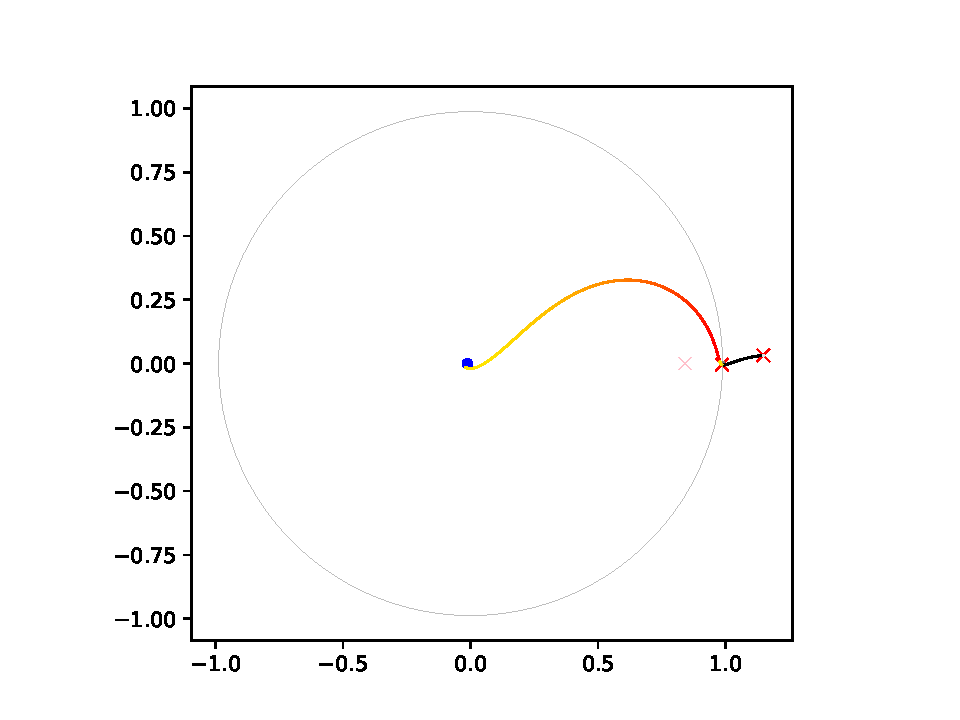
\includegraphics[width=0.46\linewidth]{fig/path_hohmann_nonin_multi_0_and_3.pdf}
        \label{fig:path_hohmann_non-inertial_multi}
    }
    \hfill
    \subfloat[The rate of separation between infinitesimally perturbed versions of the Hohmann transfer]{
        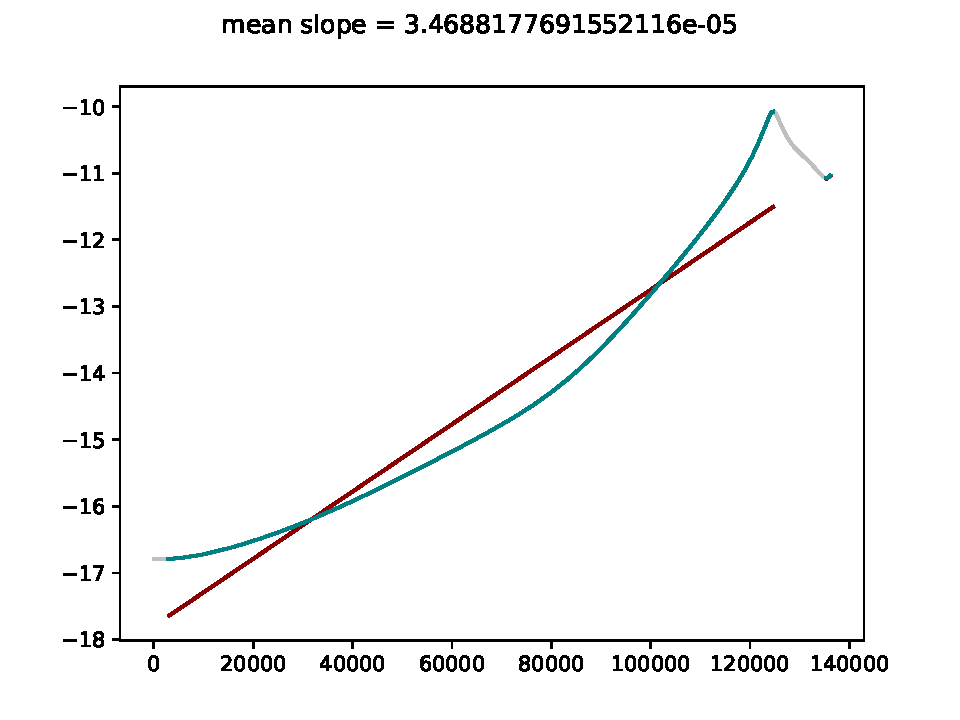
\includegraphics[width=0.46\linewidth]{fig/hohmann_slope_0_and_3}
        \label{fig:hohmann_slope}
    }
    \\
    \subfloat[A relatively long LETO path (black) and its perturbation (yellow-red gradient))]{
        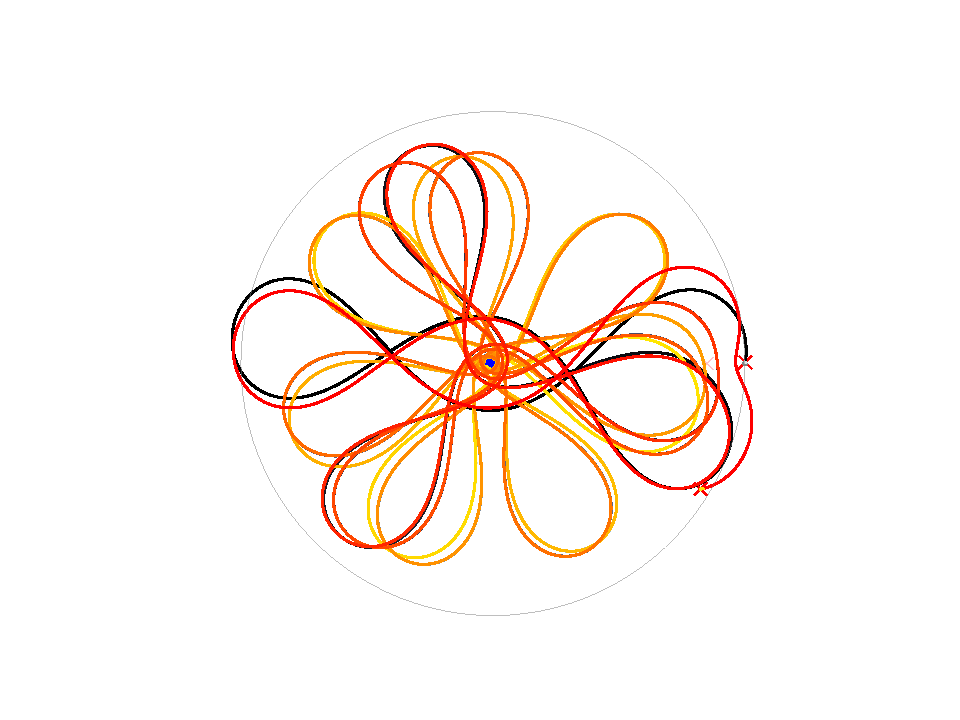
\includegraphics[width=0.46\linewidth]{fig/path_long_leto_nonin_multi_1_and_3.pdf}
        \label{fig:path_long_leto_non-inertial_multi}
    }
    \hfill
    \subfloat[The rate of separation of two infinitesimally perturbed versions of the long LETO]{
        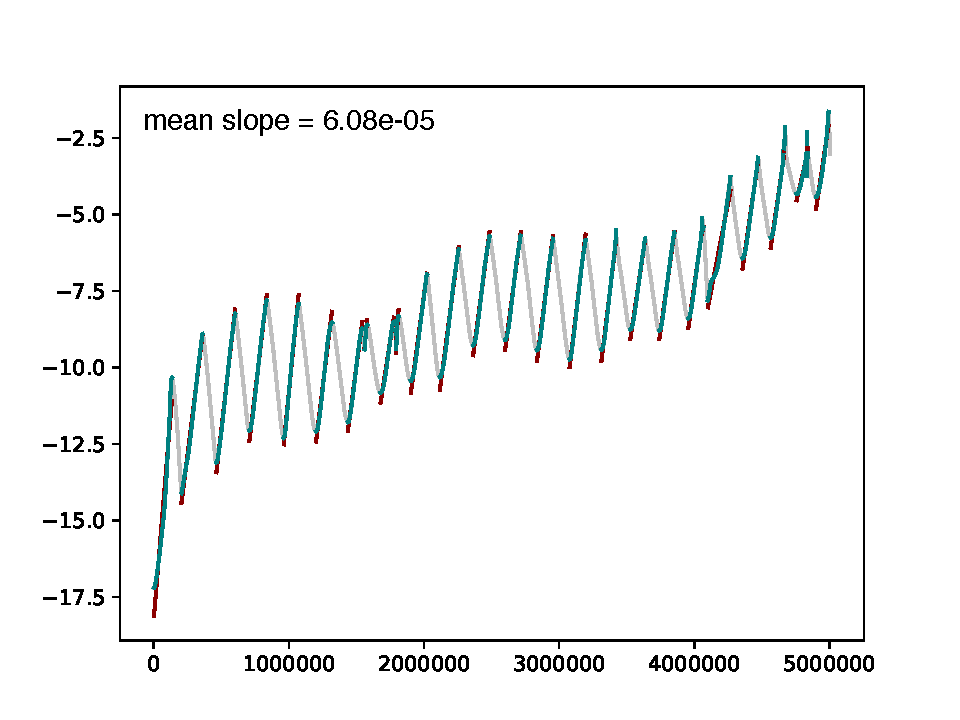
\includegraphics[width=0.46\linewidth]{fig/long_leto_slope_1_and_3}
        \label{fig:long_leto_slope}
    }
    \caption{Examples of some of the different types of transfers that are possible within the model. Each of these were taken as starting points, and simulated again with slightly perturbed starting conditions. The difference between these perturbations were then measured, and plotted in \textbf{b} and \textbf{d}, on a logarithmic scale. The slope of these plots is the lyapunov exponent. We can see that passing into a deep gravity well has a stabilizing effect on the chaos in the system.}
    \label{fig:lyapunov}
\end{figure} 

Our analysis shows that given an initial perturbation in the order of \num{1e-6}, after 200 days we have an uncertainty of 50.000 kilometers. This is a very liberal upper bound for both our error and our flight time. A definite confirmation that the system is significantly chaotic, but not enough to invalidate our results. 

A more reasonable initial perturbation on the order of \num{1e-8} (one order of magnitude greater than our error tolerance) gives us an uncertainty of less than \SI{2700}{km} after the same 200 days (before we pass the moon, which of course stops one path, and heavily diverges the other). This is very manageable for a spacecraft, since it can adjust for these imprecisions with its guidance thrusters early in the process.

The mean slope for our longer and shorter missions remain the same within a single order of magnitude, (\numrange{1e-5}{1e-4}), which is encouraging. Our conclusion with regards to the chaos of the system is that it is significant, and will need to be corrected for dynamically in an actual mission, but that it does not invalidate any trajectories that we find, since the aforementioned dynamic corrections are completely covered by modern- (and to an extent, even vintage) spacecraft capabilities.
